\documentclass[t]{beamer}
\usepackage{beamerthemesplit}
\usepackage{graphics}
\usepackage{pstricks}
\usepackage{graphicx}
\usepackage{hyperref}
\usepackage{listings}
\usepackage{subfigure}
\usepackage{multirow}
\usepackage{xspace}


\mode<presentation>
{ \usetheme{Boadilla}
  \setbeamercovered{transparent}
  \setbeamertemplate{items}[circle]
  \setbeamertemplate{theorems}[numbered]
  \setbeamertemplate{footline}[frame number]
}
 
%\useinnertheme[shadow=true]{rounded}
\useoutertheme{shadow}
\usecolortheme{whale}

\newcommand\blfootnote[1]{
  \begingroup
  \renewcommand\thefootnote{}\footnote{#1}
  \addtocounter{footnote}{-1}
  \endgroup
}

\mode
<all>

\def\answer{ANS}

\title{C Programming}
\author{WanLei Zhao}


\begin{document}
\begin{frame}
   \begin{center}
    \vspace{24pt}
    \Huge\textbf{C Programming}\blfootnote{Email: wlzhao@xmu.edu.cn, copyrights are fully preserved by the author.}\\
     \Huge{\mbox{Lab 3: }if-else and switch-case}
    \vspace{36pt}
  \end{center}
  \begin{align*}
   \vspace{18pt}
      \large{\mbox{Lecturer:}~Dr.~\mbox{Wan-Lei~~Zhao}} \\
      \large{Spring~~Semester~~2022} \\
   \vspace{30pt}
  \end{align*}
\end{frame}

\definecolor{cornblue}{HTML}{6495ED}
\definecolor{navyblue}{HTML}{000080}
\definecolor{midnblue}{HTML}{191970}
\definecolor{lghtblue}{HTML}{B0C4DE}
\setbeamercolor{background}{fg=black, bg=lghtblue}
\setbeamercolor{palette primary}{fg=white, bg=lghtblue}
\setbeamercolor{palette secondary}{fg=black, bg=cornblue}
\setbeamercolor{palette tertiary}{fg=black, bg=lghtblue}
\setbeamercolor{palette quaternary}{fg=black, bg=lghtblue}
\setbeamercolor{frametitle}{fg=black, bg=white}
\definecolor{ballblue}{rgb}{0.13, 0.67, 0.8}
\definecolor{cornflowerblue}{rgb}{0.39,0.58,0.93}
\definecolor{babyblueeyes}{rgb}{0.63, 0.79, 0.95}

\setbeamertemplate{footline}
{
  \leavevmode%
  \hbox{%
  \begin{beamercolorbox}[wd=.275\paperwidth,ht=2.25ex,dp=1ex,center]{author in head/foot}%
    \usebeamerfont{author in head/foot}\insertshortauthor
  \end{beamercolorbox}%
  \begin{beamercolorbox}[wd=.44\paperwidth,ht=2.25ex,dp=1ex,center]{title in head/foot}%
    \usebeamerfont{title in head/foot}\insertshorttitle\hspace*{3em}
    \hspace*{1ex}
  \end{beamercolorbox}%
  \begin{beamercolorbox}[wd=.285\paperwidth,ht=2.25ex,dp=1ex,center]{date/foot}%
    \usebeamerfont{title in head/foot}\hspace*{2em}
    \insertframenumber{} / \inserttotalframenumber\hspace*{1ex}
  \end{beamercolorbox}}%
  \vskip0pt
}



% preset-listing options
\lstset{
  backgroundcolor=\color{white},   
  basicstyle=\footnotesize,    
  language=c,
  breakatwhitespace=false,         
  breaklines=true,                 % sets automatic line breaking
  captionpos=b,                    % sets the caption-position to bottom
  commentstyle=\color{ballblue},    % comment style
  extendedchars=true,              
  frame=single,                    % adds a frame around the code     
  keywordstyle=\color{blue},       % keyword style
  numbers=left,                    
  numbersep=5pt,                   
  numberstyle=\tiny\color{blue}, 
  rulecolor=\color{babyblueeyes},
  stepnumber=1,              
  stringstyle=\color{black},     % string literal style
  tabsize=4,                       % sets default tabsize to 4 spaces
  title=\lstname                   
}


\section{if-else}
\label{sec:if}
\begin{frame}<beamer>
    \frametitle{Outline}
    \tableofcontents[currentsection]
\end{frame}


\begin{frame}\frametitle{if-else clause (1)}
\begin{itemize}
	\item {Read a character from input}
	\begin{enumerate}
		\item {If it is in 0$\sim$9, print out ``It is a digit''}
		\item {If it is in `a'$\sim$`z', convert it into upper case and print it out}
		\item {If it is in `A'$\sim$`Z', print it out directly}
		\item {If it is blank, print ``It is blank''}
		\item {Otherwise, print ``It is not a visible character''}
	\end{enumerate}
\end{itemize}
\end{frame}

\ifx\answer\undefined
\begin{frame}[fragile]\frametitle{if-else clause (2)}
\begin{lstlisting}[basicstyle=\large]
#include <stdio.h>
int main()
{
    char ch = ' ';
    ch = getchar();
    if(ch == ' ')
    {
        printf("It is blank\n");
    }else if(ch >= '0' && ch <= '9')
    {
        printf("It is digit\n");
    }
\end{lstlisting}
\end{frame}

\begin{frame}[fragile]\frametitle{if-else clause (3)}
\begin{lstlisting}[basicstyle=\large,firstnumber=13]
    else if(ch >= 'a' && ch <= 'z')
    {
        printf("%c", ch-32);
    }    
    else if(ch >= 'A' && ch <= 'Z')
    {
        printf("%c", ch);
    }else{
        printf("It is not visible character");
    }
    return 0;
}
\end{lstlisting}
\end{frame}
\fi

%\begin{frame}
%\frametitle{if-else clause (1)}
%\vspace{-0.15in}
%\begin{itemize}
%	\item {Convert a score (0$\sim$100) to A - E levels}
%	\begin{enumerate}
%		\item {90 - 100: A}
%		\item {80 - 89: B}
%		\item {70 - 79: C}
%		\item {60 - 69: D}
%		\item {  $<$ 60: E}
%	\end{enumerate}
%	\item {The input should be a float}
%	\item {Print out the resulting level to the screen}
%\end{itemize}
%\begin{center}
%	81 -----$>$ B
%\end{center}
%
%\end{frame}
%
%\begin{frame}
%\frametitle{if-else clause (2)}
%\vspace{-0.15in}
%	\begin{enumerate}
%		\item {\#include $<$stdio.h$>$}
%		\item {int~main(~)}
%		\item {\{}
%		\item {~~~float score = 0;}
%   		\item {~~~char grade = '0';}
%		\item {~~~printf("Please input scores: ");}
%		\item {~~~scanf("\%f", \&score);}
%		\item {~~~if(score $<$ 0 $\parallel$ score $>$ 100)}
%		\item {~~~\{}
%   		\item {~~~~~printf("Input is invalid!${\setminus}$n");}
%		\item {~~~\}}
%		\item {~~~else\{}
%		\item {~~~~~if(score $>=$ 90)}
%		\item {~~~~~~~~grade = 'A';}
%		\item {~~~~~else if(score $>=$ 80)\{}
%		\item {~~~~~~~~grade = 'B';}
%		\item {~~~~~~\}else if(score $>=$ 70)\{}
%	\end{enumerate}
%\end{frame}
%
%\begin{frame}
%\frametitle{if-else clause (2)-continued}
%\begin{enumerate}
%	\setcounter{enumi}{17}
%		\item {~~~~~~~~~grade = 'C';}
%		\item {~~~~~~\}else if(score $>=$ 60)\{}
%		\item {~~~~~~~~~grade = 'D';}
%		\item {~~~~~~\}else \{}
%		\item {~~~~~~~~~~grade = 'E';}
%		\item {~~~~~~~\}}
%		\item {~~~\}//if-else}
%		\item {~~~printf("\%5.1f ---$>$ \%c${\setminus}$n", score, grade);}
%		\item {\}}
%\end{enumerate}
%\end{frame}

\section{Embedded if-else}
\label{sec:if1}
\begin{frame}<beamer>
    \frametitle{Outline}
    \tableofcontents[currentsection]
\end{frame}

\begin{frame}
\frametitle{Embedded if-else}
\vspace{-0.1in}
\begin{itemize}
	\item {Given the height and gender of a student, recommend a sport for him/her}
\end{itemize}
\begin{figure}
	\begin{center}
		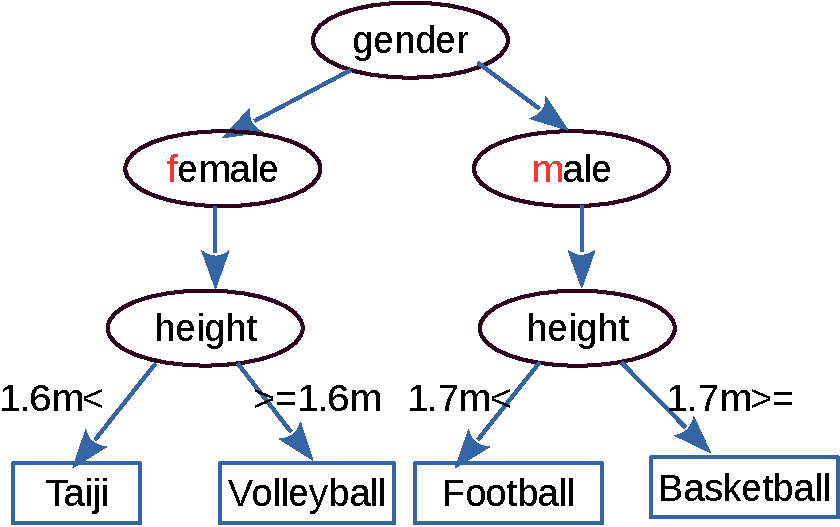
\includegraphics[width=0.45\linewidth]{figs/sports.pdf}
	\end{center}
\end{figure}
\begin{itemize}
	\item {For exapmle, given male student with height 1.75m, it is recommended to play basketball}
	\item {Th input is \textcolor{red}{m}/\textcolor{red}{f} for gender, and a positive float number for height}
	\item {The output is the recommended sports name}
\end{itemize}
\end{frame}

\ifx\answer\undefined
\begin{frame}[fragile]{The answer (1)}
\begin{lstlisting}[xleftmargin=0.05\linewidth]
#include <stdio.h>
int main( )
{
  char gender = ' ';
  float height = 0.0;
  printf("Please input gender: ");
  scanf("%c", &gender);
  printf("Please input height: ");
  scanf("%f", &height);
  if(gender == 'm')
  {
     if(height >= 1.70)
     {
         printf("Basketball\n");
     }else
\end{lstlisting}
\end{frame}
\fi

\ifx\answer\undefined
\begin{frame}[fragile]{The answer (2)}
\begin{lstlisting}[xleftmargin=0.05\linewidth, firstnumber=16]
     {
         printf("Football\n");
     }
  }else if(gender == 'f')
  {
     if(height >= 1.60)
     {
         printf("Volleyball\n");
     }else
     {
         printf("Taiji\n");
     }
  }//else-if(gender)
}

\end{lstlisting}
\end{frame}
\fi

\section{switch-case}
\label{sec:if}
\begin{frame}<beamer>
    \frametitle{Outline}
    \tableofcontents[currentsection]
\end{frame}

\begin{frame}
\frametitle{switch clause}
\begin{itemize}
	\item {Write C codes, which allows user to input number between 1 and 12 (the month)}
	\item {Then your code tells the user to which season the input month belongs}
\end{itemize}
\begin{center}
\begin{enumerate}
	\item {2---4 : Spring}
	\item {5---7 : Summer}
	\item {8---10 : Autumn}
	\item {12---1 : Winter}
\end{enumerate}
\end{center}
\end{frame}

\ifx\answer\undefined
\begin{frame}[fragile]
\begin{lstlisting}[xleftmargin=0.05\linewidth]
#include <stdio.h>
int main( )
{
  int m = 0;
  printf("Please input month: ");
  scanf("%d", &m);
  if(m < 1 || m > 12)
  {
    printf("The input is invalid!\n");}
  } else
  {
   switch(m)
   {
     case 2:
     case 3:
     case 4: printf("%d --- Spring\n", m); break;
\end{lstlisting}
\end{frame}
\fi

\ifx\answer\undefined
\begin{frame}[fragile]
	\begin{lstlisting}[xleftmargin=0.05\linewidth, firstnumber=15]
     case 5:
     case 6:
     case 7:printf("%d --- Summer\n", m); break;
     case 8:
     case 9:
     case 10:printf("%d --- Autumn\n", m); break;
     case 11:
     case 12:
     case 1: printf("%d --- Winter\n", m); break;
   }//end-switch
  }//end-else
}//end-main
	\end{lstlisting}
\end{frame}
\fi

\section{}
\end{document}
